\documentclass[14pt]{report}
\usepackage[english,russian]{babel}
\usepackage{setspace}
\usepackage[unicode]{hyperref}
\usepackage[utf8]{inputenc}
\usepackage{xcolor}
\usepackage{amsmath}
\usepackage{wasysym}
\usepackage{latexsym}
\usepackage{indentfirst}
\usepackage{mathtools}
\definecolor{linkcolor}{rgb}{0.0,0.0,0.0}
\definecolor{urlcolor}{HTML}{799B03}
\hypersetup{pdfstartview=FitH, linkcolor=linkcolor,urlcolor=urlcolor, colorlinks=true}
\usepackage[14pt]{extsizes}
\usepackage[
    left=30mm,
    top=20mm,
    right=10mm,
    bottom=20mm
]{geometry}
\usepackage{graphicx}
\usepackage{subfigure}
\usepackage{afterpage}
\usepackage{titlesec}
\usepackage{float}
\usepackage{listings}
\usepackage{csquotes}
\usepackage{mathrsfs}
\usepackage{amssymb}
\usepackage{caption}

% figure caption type changed
\captionsetup{labelsep=space}
\addto\captionsrussian{\renewcommand{\figurename}{Рисунок}}
% chapter settings
\titleformat{\chapter}[display]   
{\centering\Large\bfseries}{\chaptertitlename\ \thechapter}{10pt}{\Large}   
\titlespacing*{\chapter}{5pt}{-20pt}{30pt}

% section settings
\titleformat{\section}[block]
  {\large\bfseries}
  {\thesection\ }{0pt}{}

% settings for chapters and sections
\addto\captionsrussian{% Replace "english" with the language you use
  \renewcommand{\contentsname}%
    {\centering \large ОГЛАВЛЕНИЕ}%
  \renewcommand{\chaptername}{ГЛАВА}
  \renewcommand{\chaptertitlename}{ГЛАВА}
  \renewcommand{\bibname}{\large СПИСОК ИСПОЛЬЗОВАННОЙ ЛИТЕРАТУРЫ}
}

\renewcommand{\baselinestretch}{1.2}

\usepackage{amsfonts}
\usepackage{amsthm}
\newtheorem{theorem}{Теорема}
\newtheorem{cons}{Следствие}
\newtheorem{comment}{Замечание}

\begin{document}
\setcounter{page}{1}
\setstretch{1.0}
\thispagestyle{empty}
\newgeometry{
	left=0mm,
    top=20mm,
    right=0mm,
    bottom=20mm
}
\begin{center}
\bf
\vspace{4cm}
{
\setstretch{0.9}
\mbox{МИНИСТЕРСТВО~ОБРАЗОВАНИЯ~РЕСПУБЛИКИ~БЕЛАРУСЬ} \\~\\
\mbox{БЕЛОРУССКИЙ~ГОСУДАРСТВЕННЫЙ~УНИВЕРСИТЕТ} \\~\\
\mbox{МЕХАНИКО-МАТЕМАТИЧЕСКИЙ~ФАКУЛЬТЕТ} \\~\\
\mbox{Кафедра~дифференциальных~уравнений~и~системного~анализа} \\~\\
}
\vspace{4cm}
\bf
\mbox{О СВОЙСТВАХ РЕШЕНИЯ УРАВНЕНИЙ РИККАТИ ВЫСШИХ ПОРЯДКОВ}\\
\vspace{1cm}
\rm Курсовая работа 
\vspace{3cm}
\end{center}
\begin{tabular}{ll}
\hspace{10.5cm}
&Шпака Андрея Валерьевича~\\
&студента 2-го курса\\
&специальности 1-31 03 09\\
&<<Компьютерная математика\\
&и системный анализ>>\\~\\
&Научный руководитель:\\
&ассистент В.~И.~Громак
\end{tabular}
\vspace{4cm}
\begin{center}
Mинск, 2023
\end{center}
\clearpage
\restoregeometry
\tableofcontents
\chapter*{\large ВВЕДЕНИЕ}  
\addcontentsline{toc}{chapter}{ВВЕДЕНИЕ}
%Тут надо будет написать текст введения%
\chapter{Уравнение Риккати, общие свойства скалярного уравнения Риккати. Уравнения Риккати высших порядков. Матричные уравнения Риккати} 

\section{Определение скалярного уравнения Риккати. Общие свойства скалярного уравнения Риккати.}
Рассмотрим уравнение:

$$\dfrac{dy}{dx} = f \left( x, y \right),$$
в котором правая часть есть квадратичная функция (от искомой функции) $y$, т. е.
\begin{equation}
    \tag{$\mathbb{R}_1$}
    \dfrac{dy}{dx} = P \left( x \right) y^2 + Q \left( x \right) y + R \left( x \right).
\end{equation}
Такое уравнение называется уравнением Риккати \cite{matveev}. Будем считать, что функции $P \left( x \right)$, $Q \left( x \right)$, $R \left( x \right)$ определены и непрерывны в интервале $\left( a, b \right) \; \left( a \geqslant -\infty,\right.$ $\left.( b \leqslant +\infty \right),$ причем $P \left( x \right) \not\equiv 0$ и $R \left( x \right) \not\equiv 0$ в этом интервале (в противном случае уравнение Риккати вырождается в линейное уравнение или уравнение Бернулли).

При сделанных предположениях относительно $P \left( x \right)$, $Q \left( x \right)$ и $R \left( x \right)$ уравнение Риккати в $\mathbb{R}_1$ имеет единственное решение
\begin{equation}  \label{eq:single_solution}
    y = y \left( x \right)
\end{equation}
удовлетворяющее начальному условию:
\begin{equation}  \label{eq:initial_cond}
    y = y_{0} \; \; \text{при} \; \; x = x_{0},
\end{equation}
где $x_{0}$ принадлежит интервалу $\left( a, b \right),$ а за $y_{0}$ можно брать любое число, т. е. через каждую точку $\left( x_{0}, y_{0} \right)$ полосы

\begin{equation}  \label{eq:strip}
    a < x < b, \; \; -\infty < y < +\infty
\end{equation}
проходит одна и только одна интегральная кривая уравнения Риккати.

Действительно, всегда можно построить прямоугольник
$$ R: \; \; \left| x - x_{0} \right| \leqslant a_{1}, \; \; \left| y - y_{0} \right| \leqslant b_{1}$$
с центром в точке $\left( x_{0}, y_{0} \right),$ который целиком лежит в полосе $\left( \ref{eq:strip} \right)$. В этом прямоугольнике правая часть уравнения Риккати в $\mathbb{R}_1$ удовлетворяет обоим условиям теоремы Пикара. А тогда уравнение в $\mathbb{R}_1$ имеет единственное решение $\left( \ref{eq:single_solution} \right)$, удовлетворяющее начальному условию $\left( \ref{eq:initial_cond} \right)$. Это решение определено вообще говоря, лишь в некоторой окрестности точки $x = x_{0}.$ Существование этого решения во всем интервале непрерывности коэффициентов $P \left( x \right)$, $Q \left( x \right)$ и $R \left( x \right)$ не гарантируется.

Пример. Рассмотрим уравнение
\begin{equation} \label{eq:ex_1}
    y' = y^{2} - 2 y + 1.
\end{equation}
Здесь правая часть определена и непрерывна на всей плоскости $\left( x, y \right)$. Но из формулы общего решения
$$y = 1 - \dfrac{1}{x - C}$$
видно, что никакое из решений, входящих в эту формулу при $C \neq \infty,$ не будет определено при всех $x$. В Wolfram Mathematica решение данного уравнения выглядит следующим образом:
\begin{figure}[H]
	\captionsetup{justification=centering}
	\center{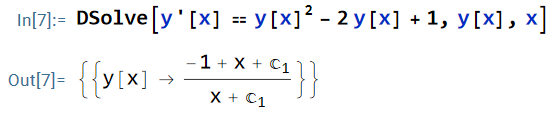
\includegraphics[width=0.7\linewidth]{pictures/wolfram-1.png}}
	\caption{Решение уравнения \eqref{eq:ex_1}}
	\label{fig:predict_gauss_proc}
\end{figure}

Из сказанного выше следует, что уравнение Риккати не имеет особых решений. Всякое решение его есть частное решение.

Выделяют следующие общие свойства скалярного уравнения Риккати.

\hypertarget{first_prop}{$1.$} Уравнение Риккати, так же, как и линейное уравнение, сохраняет свой вид при любом преобразовании независимой переменной

\begin{equation}  \label{eq:replacement}
    x = \varphi \left( t \right),
\end{equation}
где $\varphi \left( t \right)$ --- любая непрерывно-дифференцируемая функция, определенная в интервале $\left( t_{0}, t_{1} \right),$ причем $\varphi' \left( t \right) \neq 0$ в $\left( t_{0}, t_{1} \right)$ \cite{matveev}.

Действительно, так как
\begin{equation}  \label{eq:param_derivative}
    \dfrac{dy}{dt} = \dfrac{dy}{dx} \varphi'\left( t \right),
\end{equation}
то преобразованное уравнение имеет вид:
$$\dfrac{dy}{dt} = \left\{ P \left[\varphi\left( t \right) \right] y^{2} + Q \left[\varphi\left( t \right) \right] y + R\left[\varphi\left( t \right) \right] \right\} \varphi' \left( t \right),$$
т. е. является опять уравнением Риккати.

\hypertarget{sec_prop}{$2.$} В отличие от линейного уравнения, уравнение Риккати сохраняет свой вид не только при любом линейном преобразовании искомой функции, но также и при любом дробно-линейном преобразовании
\begin{equation}  \label{eq:transform}
    y = \dfrac{\alpha \left( x \right) z + \beta \left( x \right)}{\gamma \left( x \right) z + \delta \left( x \right),}
\end{equation}
где $\alpha \left( x \right), \beta \left( x \right), \gamma \left( x \right), \delta \left( x \right)$ ~--- произвольные функции, определенные и непрерывно дифференцируемые в интервале $\left( a, b \right)$, подчиненные лишь очевидному условию $\alpha \left( x \right) \delta \left( x \right) - \beta \left( x \right) \gamma \left( x \right)$ \cite{matveev}.

В самом деле, дифференцируя $\left( \ref{eq:transform} \right)$, находим:
$$ 
    y' = \dfrac{\left( \alpha'z + \alpha z' + \beta' \right) \left( \gamma z + \delta \right) - \left( \alpha z + \beta \right) \left( \gamma' z + \gamma z' + \delta \right)}{\left( \gamma z + \delta \right)^2} =
$$
\begin{equation}  \label{eq:transform_derivative}
    = \dfrac{\left( \alpha \delta - \beta \gamma \right)z' + \left( \alpha' \gamma - \alpha \gamma' \right)z^{2} + \left( \alpha' \delta' + \beta' \gamma - \alpha \delta' - \beta \gamma' \right)z + \beta' \delta - \beta \delta'}{\left( \gamma z + \delta \right)^2},
\end{equation}
так что левая часть уравнения в $\mathbb{R}_1$ заменится дробью $ \left( \ref{eq:transform_derivative} \right).$ Правая же часть уравнения в $\mathbb{R}_1$ после замены $y$ выражением $\left( \ref{eq:transform} \right)$ и приведения к общему знаменателю обратится в дробь, числитель которой есть квадратичная функция от $z,$ а знаменатель --- тот же, что и у дроби $\left( \ref{eq:transform_derivative} \right)$. Поэтому преобразованное уравнение будет опять уравнением Риккати.

Применяя то или иное из указанных преобразований, можно значительно упростить вид уравнения Риккати и, таким образом, облегчить его изучение.

$3.$ Решение уравнения Риккати не сводится, вообще говоря, к квадратурам. Однако можно установить некоторые интересные факты о его решениях \cite{egorov}.

\begin{theorem} \label{t1}
    Если известно одно частное решение уравнения Риккати, то общее его решение получается двумя квадратурами.
\end{theorem}
\begin{proof}
    Пусть $y=y_1(x)$ --- известное частное решение уравнения Риккати в $\mathbb{R}_1$, т. е.
    \begin{equation} \label{particular_solution_subst}
        \dfrac{dy_1(x)}{dx} \equiv P(x) y_1^2 + Q(x) y_1 + R(x).
    \end{equation}
    Делая замену зависимой переменной
    \begin{equation} \label{y_repl}
        y = y_1(x) + z,
    \end{equation}
    получаем уравнение относительно $z$ следующим образом:
    $$\dfrac{dy}{dx} = \dfrac{dy_1(x)}{dx} + \dfrac{dz}{dx}$$
    $$\dfrac{dz}{dx} = \dfrac{dy}{dx} - \dfrac{dy_1(x)}{dx}$$
    $$\dfrac{dz}{dx} = P(x) y^2 + Q(x) y + R(x) - P(x) y_1^2 - Q(x) y_1 - R(x)$$
    $$\dfrac{dz}{dx} = P(x) \left( y^2 - y_1^2 \right) + Q(x) \left( y - y_1 \right)$$
    $$\dfrac{dz}{dx} = P(x) \left( y_1^2 + 2 y_1 z + z^2 - y_1^2 \right) + Q(x) \left( y_1 + z - y_1 \right)$$
    $$\dfrac{dz}{dx} = P(x) z^2 + \left( 2 P y_1 + Q \right) z + R(x).$$
    
    Это уравнение Бернулли, которое заменой
    \begin{equation} \label{Bern_subst}
        z = u^{-1}
    \end{equation}
    сводится к линейному неоднородному уравнению первого порядка
    \begin{equation} \label{linear_heterog_eq_first_order}
        \dfrac{du}{dx} + \left( 2 P y_1 + Q \right) u + P = 0.
    \end{equation}
    Его общее решение находится двумя квадратурами и имеет вид
    \begin{equation} \label{solution}
        u = c \varphi(x) + \psi(x),
    \end{equation}
    где $c$ --- произвольная постоянная.

    Из формул (\ref{y_repl}) и (\ref{Bern_subst}) следует, что $u = 1/y - y_1$ и согласно формуле (\ref{solution}) отсюда получаем
    $$y = y_1 + \dfrac{1}{c \varphi(x) + \psi(x)} = \dfrac{c y_1(x) \varphi (x) + y_1(x) \psi (x) + 1}{c \varphi(x) + \psi(x)}$$
\end{proof}

Заключительная формула приведенного доказательства приводит к следующему важному выводу.
\begin{cons}
    Общее решение уравнения Риккати представляет собой дробно-линейную функцию относительно произвольной постоянной.
\end{cons}

\begin{theorem}
    Если известны два частных решения решения уравнения Риккати, то его общее решение находится одной квадратурой.
\end{theorem}
\begin{proof}
    Пусть $y_1, y_2$ --- решения уравнения Риккати в $\mathbb{R}_1$. Как показано при доказательстве теоремы \ref{t1}, замена
    \begin{equation} \label{u_subst}
        u = \dfrac{1}{y - y_1}
    \end{equation}
    сводит уравнение Риккати к неоднородному уравнению (\ref{linear_heterog_eq_first_order}). Согласно этой формуле частное решение $y_2$ уравнения в $\mathbb{R}_1$ определяет функцию
    \begin{equation}
        u_1 = \dfrac{1}{y_2 - y_1},
    \end{equation}
    которая представляет собой частное решение линейного неоднородного уравнения (\ref{linear_heterog_eq_first_order}).

    Чтобы получить еще одно частное решение этого уравнения, достаточно одной квадратуры. Построив таким образом общее решение $u$ линейного уравнения (\ref{linear_heterog_eq_first_order}), получим общее решение уравнения Риккати.
\end{proof}

\begin{theorem}
    Если известны три частных решения уравнения Риккати, то его общее решение находится без квадратур.
\end{theorem}
\begin{proof}
    Пусть $y_1, y_2, y_3$ --- частные решения уравнения Риккати. Тогда, очевидно, что функции
    \begin{equation} \label{u_1_and_u_2}
        u_1 = \dfrac{1}{y_2 - y_1}, \quad u_2 = \dfrac{1}{y_3 - y_1}
    \end{equation}
    являются частными решениями линейного неоднородного уравнения (\ref{linear_heterog_eq_first_order}). По двум частным решениям уравнения (\ref{linear_heterog_eq_first_order}) его общее решение находится без квадратур по формуле $u = u_1 + c (u_2 - u_1),$ где $c$ --- произвольная постоянная. Это решение можно представить в виде
    \begin{equation} \label{solution_without_quadratures}
        u = \dfrac{1}{y_2 - y_1} + c \left( \dfrac{1}{y_3 - y_1} - \dfrac{1}{y_2 - y_1} \right).
    \end{equation}
    С другой стороны это решение $u$ линейного уравнения можно связать с решением $y$ уравнения Риккати по формуле $u = (y - y_1)^{-1}$. Подставляя это значение в формулу (\ref{solution_without_quadratures}) и разрешив полученное соотношение относительно $c$, приходим к общему интегралу уравнения Риккати
    $$\dfrac{y - y_2}{y - y_1} : \dfrac{y_3 - y_2}{y_3 - y_1} = c$$
\end{proof}

\begin{cons}
   Двойное отношение любых четырех частных решений уравнения Риккати постоянно, т. е.
   $$\dfrac{y_4 - y_2}{y_4 - y_1} : \dfrac{y_3 - y_2}{y_3 - y_1} = c$$
\end{cons}
\begin{proof}
    Если известны четыре частных решения $y_1, y_2, y_3$ и $y_4$ уравнения Риккати, то, кроме решений (\ref{u_1_and_u_2}) линейного уравнения (\ref{linear_heterog_eq_first_order}), имеется еще и третье его решение $u_3 = (y_4 - y_1)^{-1},$ которое, очевидно, может быть также получено из формулы (\ref{solution_without_quadratures}) при некотором значении постоянной $c$. Значит, можно записать равенство
    $$\dfrac{1}{y_4 - y_1} = \dfrac{1}{y_2 - y_1} + c \left( \dfrac{1}{y_3 - y_1} - \dfrac{1}{y_2 - y_1} \right),$$
    из которого непосредственно следует справедливость утверждения.
\end{proof}

\section{Определение уравнений Риккати высших порядков.}

Уравнение Риккати $N$-го порядка зададим следующей формулой:
\begin{equation}
    \tag{$\mathbb{R}_N$}
    L^N v(x) + \sum\limits_{j=1}^N a_j(x)(L^{j - 1} v(x)) + a_0(x) = 0,
\end{equation}
где $N$ -- целое число, характеризующее порядок уравнения Риккати, $L$ -- дифференциальный оператор
$$L = \dfrac{d}{dx} + c v(x);$$
и $a_j(x) \; j = 0, 1, \dots, N$ это $N + 1$ произвольные функции \cite{chain}. Пусть $N = 1$ в формуле для $\mathbb{R}_N$. Получается уравнение Риккати первого порядка:
\begin{equation}
    \tag{$\mathbb{R}_1$}
    \dfrac{dv}{dx} + c v(x)^2 + a_1(x) v(x) + a_0(x) = 0,
\end{equation}
то есть рассмотренный выше случай.
Пусть $N = 2$ в формуле для $\mathbb{R}_N$. Можно вывести уравнение второго порядка:
$$L^2 v(x) + \sum\limits_{j=1}^2 a_j(x)(L^{j - 1} v(x)) + a_0(x) = 0,$$
$$L \left( L v(x) \right) + a_2(x) L v(x) + a_1(x) v(x) + a_0(x) = 0,$$
$$ L\left(\dfrac{dv}{dx} + cv(x)^2\right) + a_2(x) \left(\dfrac{d}{dx} + c v(x)\right) v(x) + a_1(x) v(x) + a_0(x) = 0,$$
$$ \left(\dfrac{d}{dx} + c v(x)\right)\left(\dfrac{dv}{dx} + cv(x)^2\right) + a_2(x) \dfrac{dv}{dx} + c a_2(x) v(x) + a_1(x) v(x) + a_0(x) = 0,$$
$$ \dfrac{d^2v}{dx^2} + 2c v(x) \dfrac{dv}{dx} + c v(x) \dfrac{dv}{dx} + c^2 v(x)^3 + a_2(x) \dfrac{dv}{dx} + c a_2(x) v(x) +  a_1(x) v(x) + a_0(x) = 0,$$
\begin{equation}
    \tag{$\mathbb{R}_2$}
    \dfrac{d^2v}{dx^2} + \left[ a_2(x) + 3c v(x) \right] \dfrac{dv}{dx} + c^2 v(x)^3 + c a_2(x) v(x) + a_1(x) v(x) + a_0(x) = 0.
\end{equation}
Аналогично, пусть в $N = 3$ в формуле для $\mathbb{R}_N$. Получается уравнение третьего порядка:
$$L^3 v(x) + \sum\limits_{j=1}^3 a_j(x)(L^{j - 1} v(x)) + a_0(x) = 0,$$
\begin{multline*}
    L \left( L^2 v(x) \right)+ a_3(x) L^2 v(x) + a_2(x) L v(x) + a_1(x) v(x) + a_0(x) = 0, \\
    L \left( \dfrac{d^2v}{dx^2} + 2c v(x) \dfrac{dv}{dx} + c v(x) \dfrac{dv}{dx} + c^2 v(x)^3 \right)+ a_3(x) \left( \dfrac{d^2v}{dx^2} + 2c v(x) \dfrac{dv}{dx} + c v(x) \dfrac{dv}{dx} \right. + \\ + c^2 v(x)^3 \biggr) v(x) + a_2(x) \left(\dfrac{d}{dx} + c v(x)\right) v(x) + a_1(x) v(x) + a_0(x) = 0, \\
    \left(\dfrac{d}{dx} + c v(x)\right) \left( \dfrac{d^2v}{dx^2} + 2c v(x) \dfrac{dv}{dx} + c v(x) \dfrac{dv}{dx} + c^2 v(x)^3 \right)+ a_3(x)  \dfrac{d^2v}{dx^2} + \\ + 3c a_3(x) v(x) \dfrac{dv}{dx} + c^2 a_3(x) v(x)^3 v(x) + a_2(x) \dfrac{d}{dx} + c a_2(x) v(x) + \\ + a_1(x) v(x) + a_0(x) = 0, \\
    \dfrac{d^3v}{dx^3} + 3c \left( \dfrac{dv}{dx} \right)^2 + 3c v(x) \dfrac{d^2v}{dx^2} + 3 c^2 v(x)^2 \dfrac{dv}{dx} + c v(x) \dfrac{d^2v}{dx^2} + 3 c^2 v(x)^2 \dfrac{dv}{dx} + c^3 v(x)^4 + \\ + a_3(x) \dfrac{d^2v}{dx^2} + 3c a_3(x) v(x) \dfrac{dv}{dx} + c^2 a_3(x) v(x)^3 v(x) + a_2(x) \dfrac{dv}{dx} + c a_2(x) v(x) + \\ + a_1(x) v(x) + a_0(x) = 0, \\
    \dfrac{d^3v}{dx^3} + \left[ a_3(x) + 4c v(x) \right] \dfrac{d^2v}{dx^2} + 3c \left( \dfrac{dv}{dx} \right)^2 + \left[ 6 c^2 v(x)^2 + 3c v(x) a_3(x) + a_2(x) \right] \dfrac{dv}{dx} +
\end{multline*}
\begin{equation}
    \tag{$\mathbb{R}_3$}
    + c^3 v(x)^4 + c^2 a_3(x) v(x)^3 v(x) + c a_2(x) v(x) + a_1(x) v(x) + a_0(x) = 0.
\end{equation}

\section{Общие свойства скалярного уравнения Риккати для уравнений Риккати высших порядков.}
Выполняется ли свойство \hyperlink{first_prop}{сохранения вида уравнения Риккати при любом преобразовании независимой переменной} для уравнения второго порядка?

Пусть применили замену \eqref{eq:replacement}. Вычислим вторую параметрическую производную.
Так как
\begin{equation}
\begin{aligned}[b]
    \dfrac{d^2v}{dx^2} = \dfrac{d}{dx} \left( \dfrac{dv}{dx} \right) = \dfrac{\dfrac{d}{dt} \left( \dfrac{dv}{dx} \right)}{\dfrac{dx}{dt}} = \dfrac{\dfrac{d}{dt} \left(\dfrac{\dfrac{dy}{dt}}{\dfrac{dx}{dt}}\right)}{\dfrac{dx}{dt}} = \dfrac{\dfrac{\dfrac{d^2v}{dt^2} \cdot \dfrac{dx}{dt} - \dfrac{dv}{dt} \cdot \dfrac{d^2x}{dt^2}}{\left( \dfrac{dx}{dt} \right)^2}}{\dfrac{dx}{dt}} = \\ = \dfrac{\dfrac{d^2v}{dt^2} \cdot \dfrac{dx}{dt} - \dfrac{dv}{dt} \cdot \dfrac{d^2x}{dt^2}}{\left( \dfrac{dx}{dt} \right)^3},
\end{aligned}  
\label{eq:sec_param_derivative}
\end{equation} 
то, подставив в уравнение Риккати второго порядка вместо $\dfrac{d^2v}{dx^2}$ и $\dfrac{dv}{dx}$ значения из (\ref{eq:sec_param_derivative}) и (\ref{eq:param_derivative}) соответственно, получим:
\begin{multline*}
    \dfrac{\dfrac{d^2v}{dt^2} \cdot \varphi'(t) - \dfrac{dv}{dt} \cdot \varphi''(t)}{\varphi'(t)^3} + \left[ a_2(\varphi(t)) + 3c v(\varphi(t)) \right] \dfrac{\dfrac{dv}{dt}}{\varphi'(t)} + c^2 v(\varphi(t))^3 + \\ + c a_2(\varphi(t) v(\varphi(t) + a_1(\varphi(t)) v(\varphi(t)) + a_0(\varphi(t)) = 0.
\end{multline*}
Умножим выражение на $\varphi'(t)^2$.
\begin{multline*}
    \dfrac{d^2v}{dt^2} - \dfrac{dv}{dt} \cdot \dfrac{\varphi''(t)}{ \varphi'(t)} + \left[ a_2(\varphi(t)) + 3c v(\varphi(t)) \right] \dfrac{dv}{dt} \varphi'(t) + \left( c^2 v(\varphi(t))^3 \varphi'(t)) + \right. \\ + c a_2(\varphi(t) v(\varphi(t) + a_1(\varphi(t)) v(\varphi(t)) + a_0(\varphi(t)) \big) \varphi'(t)^2 = 0,
\end{multline*}
После приведения подобных получаем уравнение
\begin{multline*}
    \dfrac{d^2v}{dt^2} + \left( \left[ a_2(\varphi(t)) + 3c v(\varphi(t)) \right] \varphi'(t) - \dfrac{\varphi''(t)}{ \varphi'(t)} \right) \dfrac{dv}{dt} + \left( c^2 v(\varphi(t))^3 \varphi'(t)) + \right. \\ + c a_2(\varphi(t) v(\varphi(t) + a_1(\varphi(t)) v(\varphi(t)) + a_0(\varphi(t)) \big) \varphi'(t)^2 = 0,
\end{multline*}
то есть опять уравнение Риккати в $\mathbb{R}_2$.

Аналогично проводится проверка выполнения свойства для уравнения третьего порядка. Находим производную:
\begin{equation}
\begin{aligned}[b]
    \dfrac{d^3v}{dx^3} = \dfrac{d}{dx} \left( \dfrac{d^2v}{dx^2} \right) = \dfrac{\dfrac{d}{dt} \left( \dfrac{d^2v}{dx^2} \right)}{\dfrac{dx}{dt}} = \dfrac{\dfrac{d}{dt} \left(\dfrac{\dfrac{d^2v}{dt^2} \cdot \dfrac{dx}{dt} - \dfrac{dv}{dt} \cdot \dfrac{d^2x}{dt^2}}{\left( \dfrac{dx}{dt} \right)^3}\right)}{\dfrac{dx}{dt}} = \\ = \dfrac{\dfrac{\left( \dfrac{d^3v}{dt^3} \cdot \dfrac{dx}{dt} - \dfrac{dv}{dt} \cdot \dfrac{d^3x}{dt^3} \right) \dfrac{dx}{dt} - 3 \left( \dfrac{d^2v}{dt^2} \cdot \dfrac{dx}{dt} - \dfrac{dv}{dt} \cdot \dfrac{d^2x}{dt^2} \right) \dfrac{d^2x}{dt^2}}{\left( \dfrac{dx}{dt} \right)^4}}{\dfrac{dx}{dt}} = \\ = \dfrac{\left( \dfrac{d^3v}{dt^3} \cdot \dfrac{dx}{dt} - \dfrac{dv}{dt} \cdot \dfrac{d^3x}{dt^3} \right) \dfrac{dx}{dt} - 3 \left( \dfrac{d^2v}{dt^2} \cdot \dfrac{dx}{dt} - \dfrac{dv}{dt} \cdot \dfrac{d^2x}{dt^2} \right) \dfrac{d^2x}{dt^2}}{\left( \dfrac{dx}{dt} \right)^5.}
\end{aligned}  
\label{eq:third_param_derivative}
\end{equation}
Подставляя в уравнение Риккати третьего порядка вместо $\dfrac{d^3v}{dx^3}$, $\dfrac{d^2v}{dx^2}$ и $\dfrac{dv}{dx}$ значения из (\ref{eq:third_param_derivative}), (\ref{eq:sec_param_derivative}) и (\ref{eq:param_derivative}) соответственно, получим:
\begin{multline*}
    \dfrac{\left( \dfrac{d^3v}{dt^3} \cdot \varphi'(t) - \dfrac{dv}{dt} \cdot \varphi'''(t) \right) \varphi'(t) - 3 \left( \dfrac{d^2v}{dt^2} \cdot \varphi'(t) - \dfrac{dv}{dt} \cdot \varphi''(t) \right) \varphi''(t)}{\varphi'(t)^5} + \\ + \left[ a_3(x) + 4c v(x) \right] \dfrac{\dfrac{d^2v}{dt^2} \cdot \varphi'(t) - \dfrac{dv}{dt} \cdot \varphi''(t)}{ \varphi'(t)^3} + 3c \left( \dfrac{\dfrac{dv}{dt}}{\varphi'(t)} \right)^2 + \\ + \left[ 6 c^2 v(x)^2 + 3c v(x) a_3(x) + a_2(x) \right] \dfrac{\dfrac{dv}{dt}}{\varphi'(t)} + \\ + c^3 v(x)^4 + c^2 a_3(x) v(x)^3 v(x) + c a_2(x) v(x) + a_1(x) v(x) + a_0(x) = 0,
\end{multline*}
Умножим выражение на $\varphi'(t)^3$.
\begin{multline*}
    \dfrac{d^3v}{dt^3} - \dfrac{dv}{dt} \cdot \dfrac{\varphi'''(t)}{\varphi'(t)} - 3 \dfrac{d^2v}{dt^2} \cdot \dfrac{\varphi''(t)}{\varphi(t)} - 3 \dfrac{dv}{dt} \cdot \left( \dfrac{\varphi''(t)}{\varphi'(t)} \right)^2  + \left[ a_3(x) + 4c v(x) \right] \dfrac{d^2v}{dt^2} \cdot \varphi'(t) - \\ - \left[ a_3(x) + 4c v(x) \right] \dfrac{dv}{dt} \cdot \varphi''(t) + 3c \left( \dfrac{dv}{dt} \right)^2 \cdot \varphi'(t) + \left[ \right. 6 c^2 v(x)^2 + 3c v(x) a_3(x) + \\ + a_2(x) \left. \right] \dfrac{dv}{dt} \cdot \varphi'(t)^2 + \left( \right. c^3 v(x)^4 + c^2 a_3(x) v(x)^3 v(x) + c a_2(x) v(x) + \\ + a_1(x) v(x) + a_0(x) \big) \cdot  \varphi'(t)^3 = 0.
\end{multline*}
После приведения подобных получаем уравнение
\begin{multline*}
    \dfrac{d^3v}{dt^3} + \left( \left[ a_3(x) + 4c v(x) \right ] \cdot \varphi'(t) - 3 \cdot \dfrac{\varphi''(t)}{\varphi(t)} \right) \dfrac{d^2v}{dt^2} + 3c \left( \dfrac{dv}{dt} \right)^2 \cdot \varphi'(t) + \\ + \left( \right. \left[ \right. 6 c^2 v(x)^2 + 3c v(x) a_3(x) + a_2(x) \left. \right] \cdot \varphi'(t)^2 - \left[ a_3(x) + 4c v(x) \right] \cdot \varphi''(t) - \dfrac{\varphi'''(t)}{\varphi'(t)} \left. \right) \dfrac{dv}{dt} + \\ + \left( \right. c^3 v(x)^4 + c^2 a_3(x) v(x)^3 v(x) + c a_2(x) v(x) + a_1(x) v(x) + a_0(x) \big) \cdot \left( \varphi'(t) \right)^3 = 0,
\end{multline*}
что снова является уравнением Риккати в $\mathbb{R}_3$

 Сохраняет ли свой вид уравнение Риккати в $\mathbb{R}_2$ при \hyperlink{sec_prop}{любом дробно-линейном преобразовании} \eqref{eq:transform}? Пусть, как и в случае \eqref{eq:transform} для скалярного уравнения Риккати в $\mathbb{R}_1$, есть замена функции $v(x)$ дробно-линейным выражением для уравнений высших порядков:
 \begin{equation}  \label{eq:v_transform}
    v = \dfrac{\alpha \left( x \right) z + \beta \left( x \right)}{\gamma \left( x \right) z + \delta \left( x \right).}
\end{equation}
Тогда производная функции $v(x)$ примет вид:
\begin{equation}  \label{eq:v_transform_derivative}
    v' = \dfrac{\left( \alpha \delta - \beta \gamma \right)z' + \left( \alpha' \gamma - \alpha \gamma' \right)z^{2} + \left( \alpha' \delta' + \beta' \gamma - \alpha \delta' - \beta \gamma' \right)z + \beta' \delta - \beta \delta'}{\left( \gamma z + \delta \right)^2}.
\end{equation}
 Дифференцируя \eqref{eq:v_transform_derivative}, находим:
\begin{multline*}
    v'' = \left( \dfrac{\left( \alpha \delta - \beta \gamma \right)z' + \left( \alpha' \gamma - \alpha \gamma' \right)z^{2} + \left( \alpha' \delta' + \beta' \gamma - \alpha \delta' - \beta \gamma' \right)z + \beta' \delta - \beta \delta'}{\left( \gamma z + \delta \right)^2} \right)',\\
    v'' = \dfrac{\left( (\alpha \delta - \beta \gamma)z' + (\alpha' \gamma - \alpha \gamma')z^{2} + ( \alpha' \delta' + \beta' \gamma - \alpha \delta' - \beta \gamma')z + \beta' \delta - \beta \delta' \right)' \left( \gamma z + \right.}{\left( \gamma z + \delta \right)^4} \\ \dfrac{+ \delta \big)^2 - \left( (\alpha \delta - \beta \gamma)z' + (\alpha' \gamma - \alpha \gamma')z^{2} + ( \alpha' \delta' + \beta' \gamma - \alpha \delta' - \beta \gamma')z + \beta' \delta - \right.}{} \\ \dfrac{- \beta \delta' \big) \left( \left( \gamma z + \right. \right. \delta \big)^2 \big)'}{},
\end{multline*}
\begin{equation}
\begin{aligned}[b]
    v'' = \dfrac{\left( \right. 2 \left( \alpha' \delta - \beta \gamma' \right)z' + \left( \alpha \delta - \beta \gamma \right)z'' + \left( \alpha'' \gamma - \alpha \gamma''\right)z^{2} + }{\left( \gamma z + \delta \right)^4} \\ \dfrac{+ 2 \left( \alpha' \gamma - \alpha \gamma'\right)z z' + \left( \alpha'' \delta' + \alpha' \delta'' + \beta'' \gamma - \alpha' \delta' -\alpha \delta'' - \beta \gamma'' \right)z + }{} \\ \dfrac{ + \beta'' \delta -\beta \delta'' \big) (\gamma z + \delta)^2 - 2\left( (\alpha \delta - \beta \gamma)z' + (\alpha' \gamma - \alpha \gamma')z^{2} + \right.}{} \\ \dfrac{+ ( \alpha' \delta' + \beta' \gamma - \alpha \delta' - \beta \gamma')z + \beta' \delta  - \beta \delta' \big) \left( \gamma z +  \delta \right) \left( \gamma' z + \gamma z' +  \delta' \right)}{},
\end{aligned}  
\label{eq:v_sec_transform_derivative}
\end{equation}
так что $\dfrac{d^2v}{dx^2}$ в уравнении $\mathbb{R}_2$ заменим дробью \eqref{eq:v_sec_transform_derivative}, $\dfrac{dv}{dx}$ заменим на \eqref{eq:v_transform_derivative}. В оставшейся же части уравнения заменим $v(x)$ на \eqref{eq:v_transform}: 
\begin{multline*}
    \dfrac{\left( \right. 2 \left( \alpha' \delta - \beta \gamma' \right)z' + \left( \alpha \delta - \beta \gamma \right)z'' + \left( \alpha'' \gamma - \alpha \gamma''\right)z^{2} + }{\left( \gamma z + \delta \right)^4} \\ \dfrac{+ 2 \left( \alpha' \gamma - \alpha \gamma'\right)z z' - \left( \alpha'' \delta' + \alpha' \delta'' + \beta'' \gamma - \alpha' \delta' -\alpha \delta'' - \beta \gamma'' \right)z + }{} \\ \dfrac{ + \beta'' \delta -\beta \delta'' \big) (\gamma z + \delta)^2 - 2\left( (\alpha \delta - \beta \gamma)z' + (\alpha' \gamma - \alpha \gamma')z^{2} + \right.}{} \\ \dfrac{+ ( \alpha' \delta' + \beta' \gamma - \alpha \delta' - \beta \gamma')z + \beta' \delta  - \beta \delta' \big) \left( \gamma z +  \delta \right) \left( \gamma' z + \gamma z' +  \delta' \right)}{} + \\ +  \dfrac{\left( \alpha \delta - \beta \gamma \right)z' + \left( \alpha' \gamma - \alpha \gamma' \right)z^{2} + \left( \alpha' \delta' + \beta' \gamma - \alpha \delta' - \beta \gamma' \right)z + \beta' \delta - \beta \delta'}{\left( \gamma z + \delta \right)^2} + \\ + c^2 \left( \dfrac{\alpha z + \beta }{\gamma z + \delta} 
 \right)^3 + c a_2(x) \dfrac{\alpha z + \beta }{\gamma z + \delta}  + a_1(x) \dfrac{\alpha z + \beta }{\gamma z + \delta}  + a_0(x) = 0.
\end{multline*}
Умножим уравнение на $\left( \gamma z + \delta \right)^4$:
\begin{multline*}
    \left( \right. 2 \left( \alpha' \delta - \beta \gamma' \right)z' + \left( \alpha \delta - \beta \gamma \right)z'' + \left( \alpha'' \gamma - \alpha \gamma''\right)z^{2} + 2 \left( \alpha' \gamma - \alpha \gamma'\right)z z' + \\ + \left( \alpha'' \delta' + \alpha' \delta'' + \beta'' \gamma - \alpha' \delta' -\alpha \delta'' - \beta \gamma'' \right)z + \beta'' \delta -\beta \delta'' \big) (\gamma z + \delta)^2 - \\ - 2\left( (\alpha \delta - \beta \gamma)z' + (\alpha' \gamma - \alpha \gamma')z^{2} + \right. ( \alpha' \delta' + \beta' \gamma - \alpha \delta' - \beta \gamma')z + \beta' \delta - \\ - \beta \delta' \big) \left( \gamma z +  \delta \right) \left( \gamma' z + \gamma z' +  \delta' \right) +  \left( \right. \left( \alpha \delta - \beta \gamma \right)z' + \left( \alpha' \gamma - \alpha \gamma' \right)z^{2} + \\ + \left( \alpha' \delta' + \beta' \gamma - \alpha \delta' - \beta \gamma' \right)z + \beta' \delta - \beta \delta' \big) \left( \gamma z + \delta \right)^2 + c^2 \left( \alpha z + \beta \right)^3 (\gamma z + \delta) + \\ + c a_2(x) (\alpha z + \beta) (\gamma z + \delta)^3  + a_1(x) (\alpha z + \beta) (\gamma z + \delta)^3  + a_0(x) (\gamma z + \delta)^4 = 0.
\end{multline*}
Преобразованное уравнение будет опять уравнением Риккати в $\mathbb{R}_2$. Для уравнения третьего порядка проверка этого свойства выполняется аналогичным образом.
\section{Определение матричного дифференциальное уравнения Риккати. Свойства матричного уравнения Риккати.}
Матричное уравнение Риккати определяется как
\begin{equation} \label{eq:matrix_eq}
    \dot X = Q(t) + A(t)X + X B(t) + X R(t) X,
\end{equation}
где $Q(t), A(t), B(t)$ и $R(t)$ --- заданные $n$-квадратные матрицы, определенные на некотором (конечном или бесконечном) отрезке времени $t$, $X$ --- искомая $n$-квадратная матрица \cite{egorov}.

Выделяют следующие свойства матричного уравнения Риккати:

1. Аналогично свойству скалярного уравнения и уравнений высших порядков, тип уравнения не изменяется при замене независимой переменной
\begin{equation}
    t = \varphi(\tau),
\end{equation}
где $\varphi(\tau)$ --- произвольная дифференцируемая функция \cite{egorov}.

2. Если матрица $R^{-1}$ существует, то заменой $Y = RX$ уравнение \eqref{eq:matrix_eq} приводится к виду
\begin{equation} \label{eq:_matrix_eq_ric_form}
    \dot Y = Q_1 (t) + A_1(t) Y + Y B_1(t) + Y^2,
\end{equation}
где $Q_1 = RQ, A_1 = (RA + \dot R) R^{-1}, B_1 = B.$

Действительно. Если обе части уравнения \eqref{eq:matrix_eq} умножить слева на $R$ и ввести соответствующие обозначения, то получим уравнение \eqref{eq:_matrix_eq_ric_form} \cite{egorov}.

3. Аналогично теоремам скалярного уравнения Риккати, выделим ряд важных свойств, показывающих, что матричное уравнение сводится к линейному, а отношение любых четырех частных решений матричного уравнения Риккати есть постоянная матрица \cite{egorov}.

Замена переменной
\begin{equation}
    Y = Z - B_1
\end{equation}
уравнение \eqref{eq:_matrix_eq_ric_form} приводит к виду
\begin{equation}
    \dot Z = Q_2 + A_2 Z + Z^2,
\end{equation}
где $A_2 = A_1 - B_1, Q_2 = Q_1 - A_1 B + \dot B_1.$

Аналогично заменой
\begin{equation}
    Y = Z - A_1
\end{equation}
уравнение \eqref{eq:_matrix_eq_ric_form} приводится к виду
\begin{equation}
    \dot Z = Q_3 + Z B_3 + Z^2,
\end{equation}
где $B_3 = B1 - A_1, Q_3 = Q_1 - A_1 B_{1}^{2} - \dot A_1.$
\begin{theorem} \label{matrix_theorem_1}
    Если $X = X_1(t)$ --- частное решение уравнения \eqref{eq:matrix_eq}, то заменой
    \begin{equation} \label{eq:repl_2}
        X = Y + X_1
    \end{equation} 
    это уравнение сводится к уравнению Бернулли
    \begin{equation} \label{eq:matrix_to_bern}
        \dot Y = A_3 Y + Y B_3 + Y R Y,
    \end{equation}
    где
    \begin{equation} \label{eq:a3_b3}
        A_3 = A + X_1 R, B_3 = B + R X_1, 
    \end{equation}
\end{theorem}
\begin{proof}
    Так как $X = X_1(t)$ --- решение уравнения \eqref{eq:matrix_eq}, то справедливо тождество
    \begin{equation}
    \dot X_1(t) \equiv Q(t) + A(t) X_1(t) + X_1(t) B(t) + X_1(t) R(t) X_1(t).
    \end{equation}
    Поэтому, подставляя замену \eqref{eq:repl_2} в уравнение \eqref{eq:matrix_eq}, получим уравнение \eqref{eq:matrix_to_bern}.
\end{proof}
\begin{theorem} \label{matrix_theorem_2}
    Если $X_1$ --- частное решение уравнения \eqref{eq:matrix_eq}, а $Z = Z_1(t)$ и $U = U_1(t)$ --- неособенные решения уравнений
    \begin{equation} \label{eq:z_point}
        \dot Z = - B_3(t) Z,
    \end{equation}
    \begin{equation} \label{eq:u_point}
        \dot U = -U A_3 (t)
    \end{equation}
    соответственно, где матрицы $A_3$ и $B_3$ определяются формулами \eqref{eq:a3_b3}, то общее решение уравнения \eqref{eq:matrix_eq} находится одной квадратурой.
\end{theorem}
\begin{proof}
    В соответствии с теоремой \ref{matrix_theorem_1} уравнение \eqref{eq:matrix_eq} сводим к уравнению Бернулли \eqref{eq:matrix_to_bern} заменой $X = Y + X_1$. Как отмечалось выше, уравнение \eqref{eq:matrix_to_bern} сводится к линейному уравнению
    \begin{equation} \label{eq:bern_to_linear}
        \dot V + B_3 V + V A_3 = - R
    \end{equation}
    с помощью замены
    \begin{equation}
        V = Y^{-1}.
    \end{equation}
    
    Общее решение уравнения \eqref{eq:bern_to_linear} можно представить в виде
    \begin{equation}
        V = V^0 + V_1,
    \end{equation}
    где $V_1$ --- частное решение этого уравнения, а $V^0$ --- общее решение соответствующего однородного уравнения
    \begin{equation} \label{eq:theta}
        \dot W + B_3(t) W + W A_3(t) = \theta.
    \end{equation}
    Общее решение этого уравнения можно представить в виде
    \begin{equation} \label{eq:v_0}
        V^0 = Z_1(t) C U_1(t),
    \end{equation}
    где $C$ --- произвольная постоянная матрица, а $Z_1(t)$ и $U_1(t)$ --- неособенные решения уравнений \eqref{eq:z_point} и \eqref{eq:u_point}. Зная общее решение \eqref{eq:v_0} уравнения \eqref{eq:theta}, можем определить частное решение $V_1$ неоднородного уравнения \eqref{eq:bern_to_linear} методом вариации постоянной $C$.

    Если теперь в цепочке преобразований переменных, которые использовались в ходе доказательства теоремы, вернуться к исходной переменной $X$, то можно определить структуру решения исходного уравнения Риккати в зависимости от произвольной постоянной матрицы $C$:
    \begin{equation} \label{eq:back_to_x}
        X = (Z_1 C U_1 + V_1)^{-1} + X_1.
    \end{equation}
\end{proof}
\begin{theorem}
    Пусть $X_1, X_2, X_3$ и $X_4$ --- частные решения уравнения \eqref{eq:matrix_eq}, а $U(t)$ --- неособеное решение уравнения
    \begin{equation}
        \dot U + U A_3(t) = 0,
    \end{equation}
    где $A_3$ определяется формулой \eqref{eq:a3_b3}.

    Тогда существует постоянная матрица $C_0$ такая, что
    \begin{equation} \label{eq:c_0}
        U(X_4 - X_1) (X_4 - X_2)^{-1}(X_3 - X_2)(X_3 - X_1)^{-1} U^{-1} = C_0.
    \end{equation}
\end{theorem}
\begin{proof}
    В соотеветствии с теоремой \eqref{matrix_theorem_2} общее решение уравнения \eqref{eq:matrix_eq} можно представить в виде \eqref{eq:back_to_x}. Придавая матрице $C$ конкретные значения, определим решения $X_2, X_3$ и $X_4$ в форме $X_i = (Z C_i U + V)^{-1} + X_1$, $i = 2, 3, 4.$

    Отсюда получаем $(X_i - X_1)(Z C_i U + U) = E$, $i, j = 2, 3, 4,$ где $E$ --- единичная матрица и поэтому
    \begin{equation} \label{eq:some_eq}
        Z(C_i - C_j) = [(X_i - X_1)^{-1} - (X_j - X_i)^{-1}] U^{-1}, i, j = 2, 3, 4, i \neq j.
    \end{equation}
    Равенства \eqref{eq:some_eq} можно представить в виде
    \begin{equation}
        Z(C_i - C_j) = (X_i - X_1)^{-1}(X_j - X_i)(X_j - X_1)^{-1} U^{-1}.
    \end{equation}

    Следовательно, справедливы равенства
    \begin{equation}
        Z(C_2 - C_3) = (X_2 - X_1)^{-1}(X_3 - X_2)(X_3 - X_1)^{-1} U^{-1},
    \end{equation}
    \begin{equation}
        Z(C_2 - C_4) = (X_2 - X_1)^{-1}(X_4 - X_2)(X_4 - X_1)^{-1} U^{-1}.
    \end{equation}

    Предполагая, что матрицы $C_2 - C_1$ и $C_2 - C_4$ обратимы, получаем равненство
    \begin{multline*}
        (X_3 - X_2)(X_3 - X_1)^{-1} U^{-1}(C_2 - C_3)^{-1} = \\ = (X_4 - X_2)(X_4 - X_1)^{-1} U^{-1} (C_2 - C_4)^{-1}.
    \end{multline*}
    Отсюда получаем равенство \eqref{eq:c_0}, в котором $C_0 = (C_2 - C_4)^{-1} (C_2 - C_3).$
\end{proof}
\begin{comment}
    В Формуле \eqref{eq:some_eq} использовано решение $U$ уравнения \eqref{eq:u_point}. Однако можно получить аналогичную формулу, в которой вместо $U$ фигурирует решение $Z$ уравнения \eqref{eq:z_point}. Точнее, тем же способом можно доказать справедливость соотношения
    $$Z^{-1} (X_3 - X_1)^{-1} (X_3 - X_2)(X_4 - X_2)^{-1}(X_4 - X_1) Z = C,$$
    где $C$ --- постоянная матрица.
\end{comment} 
%\chapter{Определения  матричных уравнений Риккати и уравнений Риккати высших порядков}%
%\section{Тут может быть заголовок 1.}%

%\section{Тут может быть заголовок 2.}%

%\chapter{Основные свойства матричных уравнений Риккати и уравнений Риккати высших порядков из цепочки.}%

%\section{Тут может быть заголовок 1.}%

%\section{Тут может быть заголовок 2.}%

%\chapter{Анализ и сравнение основных свойств решений скалярного уравнения Риккати и матричных уравнений Риккати и уравнений Риккати высших порядков из цепочки.}%
%\section{Тут может быть заголовок 1.}%

%\section{Тут может быть заголовок 2.}%
\chapter*{ \large ЗАКЛЮЧЕНИЕ}
\addcontentsline{toc}{chapter}{ЗАКЛЮЧЕНИЕ}
%Тут надо будет написать текст заключения%
%\chapter*{\large СПИСОК ИСПОЛЬЗОВАННОЙ ЛИТЕРАТУРЫ}
\begin{thebibliography}{99}
\bibitem{em} Матвеев Н.~М. Методы интегрирования ОДУ. 1974.
\bibitem{em} Егоров А.~И. Обыкновенные дифференциальные уравнения с приложениями. 2005.
\bibitem{em} Grundland A.~M., D.Levi. Higher Order Riccati Equations as Backlund Transformations, CRM-2469. 1997.
\bibitem{em} Пакет Mathematica. Вольфрам.

\end{thebibliography}
\addcontentsline{toc}{chapter}{СПИСОК ИСПОЛЬЗОВАННОЙ ЛИТЕРАТУРЫ}
\titleformat{\section}[block]
  {\large\bfseries\centering}
  {\thesection\ }{}{}
\chapter*{ПРИЛОЖЕНИЕ А}
%\addcontentsline{toc}{chapter}{ПРИЛОЖЕНИЕ А}
%\section*{\centering Код программы. Модель автокодировщика}%

%\chapter*{ПРИЛОЖЕНИЕ Б}%
%\addcontentsline{toc}{chapter}{ПРИЛОЖЕНИЕ Б}
%\section*{\centering Код программы. Обучение автокодировщика}%

%\chapter*{ПРИЛОЖЕНИЕ В}%
%\addcontentsline{toc}{chapter}{ПРИЛОЖЕНИЕ В}
%\section*{\centering Код программы. Гауссовский процесс и байесовская оптимизаия}%
\end{document}

\grid
